\chapter{Analysis of Neutrino Interactions in a Liquid Argon Time-Projection Chamber}\label{chapter:Analysis}
\section{Introduction}
The goal of this thesis is to demonstrate a fully automated reconstruction chain for event data from \ac{LAr TPC}s. Since the details of charge readout and position reconstruction will vary depending on the detector technology and geometry, as well as the equipment used, this study begins from the point at which three-dimensional hit data exists in a persistent on-disk format. This chapter uses the algorithms and techniques presented earlier to attempt to reconstruct physics information such as the muon energy from charged current $\nu_\mu$ interactions at beam energies of $770\MeV$ and $4.5\GeV$.

\section{Charged Current $\nu_\mu \rightarrow \mu + p$ at $770\MeV$}
\subsection{Event Selection Efficiency}
A sample of $1000$ events produced from charged current interactions of $\nu_\mu$ at $770\MeV$, yielding $\mu + p$ (only) final states were considered. These are the same events used for validation of algorithms earlier in this thesis. Of these 1000 events, 878 survive the initial requirement that the true proton track has more than 20 hits and undergo reconstruction. After reconstruction, 420 events have only two tracks in the output (events with more tracks in the output can potentially be recovered with improved merging algorithms, or by discarding delta electron tracks). Of these, 407 events have at least one output track containing over 1000 hits (of which, 10 events have both tracks with over 1000 hits). In 341 events, there is one track with over 1000 hits, and one smaller track. The long track is identified from the truth information as corresponding to the muon, and the shorter track is identified from the truth information as corresponding to the proton.

Based on the numbers above, an analysis that required precisely two tracks, one of which had over 1000 hits, and the other with fewer than 1000 hits will recover 397 events from the sample of 1000, of which 341 will be correctly identified as $\mu + p$ events, with the tracks tagged with the right particle type. This corresponds to an efficiency of $397/1000 = 39.7\%$ for selecting $\mu + p$ events, with a purity of $341/397 = 85.9\%$.

While the efficiency of this selection is low (under $40\%$), the purity attained is high (over $85\%$), and as already mentioned it is possible to recover many more events with improvements to the reconstruction chain.

\subsection{Muon Energy Reconstruction}
\subsubsection{Using Number of Hits}
In an ideal scenario, the number of hits in a cluster should correspond approximately to the length of the cluster in $\mm$. Since the range of a muon track varies with the initial energy of the muon, assuming minimum-ionising behaviour throughout, it should be possible to obtain a calibration for conversion between number of hits (or muon track length) and initial muon energy. In practice, the number of hits in an output cluster is a poor estimator for the initial muon energy, as demonstrated in figure \ref{fig:ccqe-770-e-nhits-calib}. One possible reason for this is the loss of hits in the cellular automaton state of the reconstruction; the proportion of lost hits rises with track length, resulting in increasingly poor estimates. However, since the hit loss should occur throughout the track, it may be possible to use the length itself to estimate the energy.

\begin{figure}
    \centering
    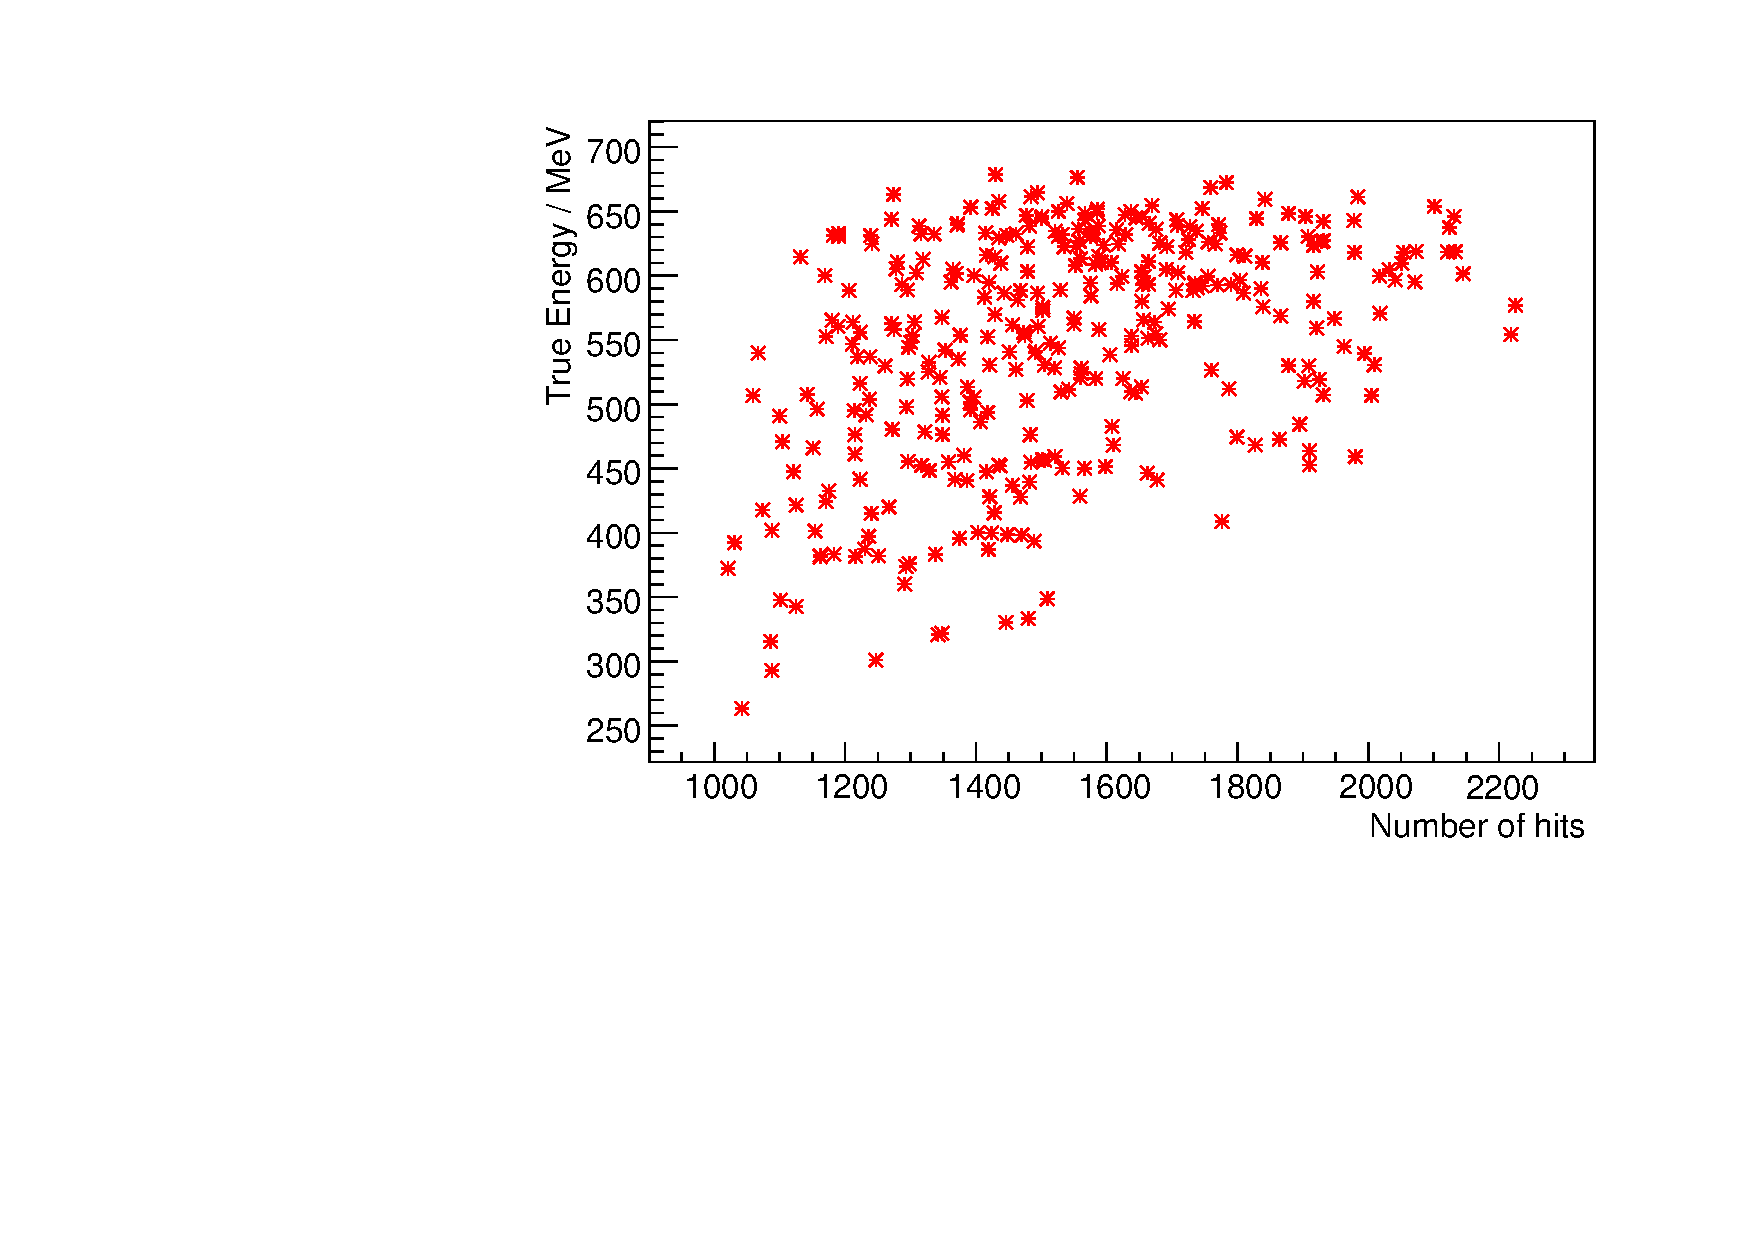
\includegraphics[angle=-90,width=0.8\textwidth]{chapters/analysis_images/ccqe-770-e-nhits-calib}
    \caption[Relationship between number of hits and energy]{\label{fig:ccqe-770-e-nhits-calib}The relationship between the number of hits $N$ in a muon cluster and the initial energy $E_\mu$ of the particle, in $\MeV$. The broad distribution indicates that the number of hits is not a good estimator for the energy of the particle, and that calibrations based on this quantity cannot provide reliable energy estimates.}
\end{figure}

\subsubsection{Using Track Length}
Calculating the length of the track is not as simple as taking the ``smallest'' and ``largest'' hits and determining the distance between them, since it is possible that the muon track may undergo significant scattering along its length, and can develop an appreciable curve. In order to determine the track length, an algorithm must run along the track in small steps, adding up the segment lengths as it goes. Such a mechanism can be easily implemented using the \ac{KDTree} structure described in chapter \ref{sec:latte_kdtree}, but this introduces another parameter; the radius used for the neighbour search, which becomes the maximum segment length.

\begin{figure}
    \centering
    \subfigure[$20\mm$]{
        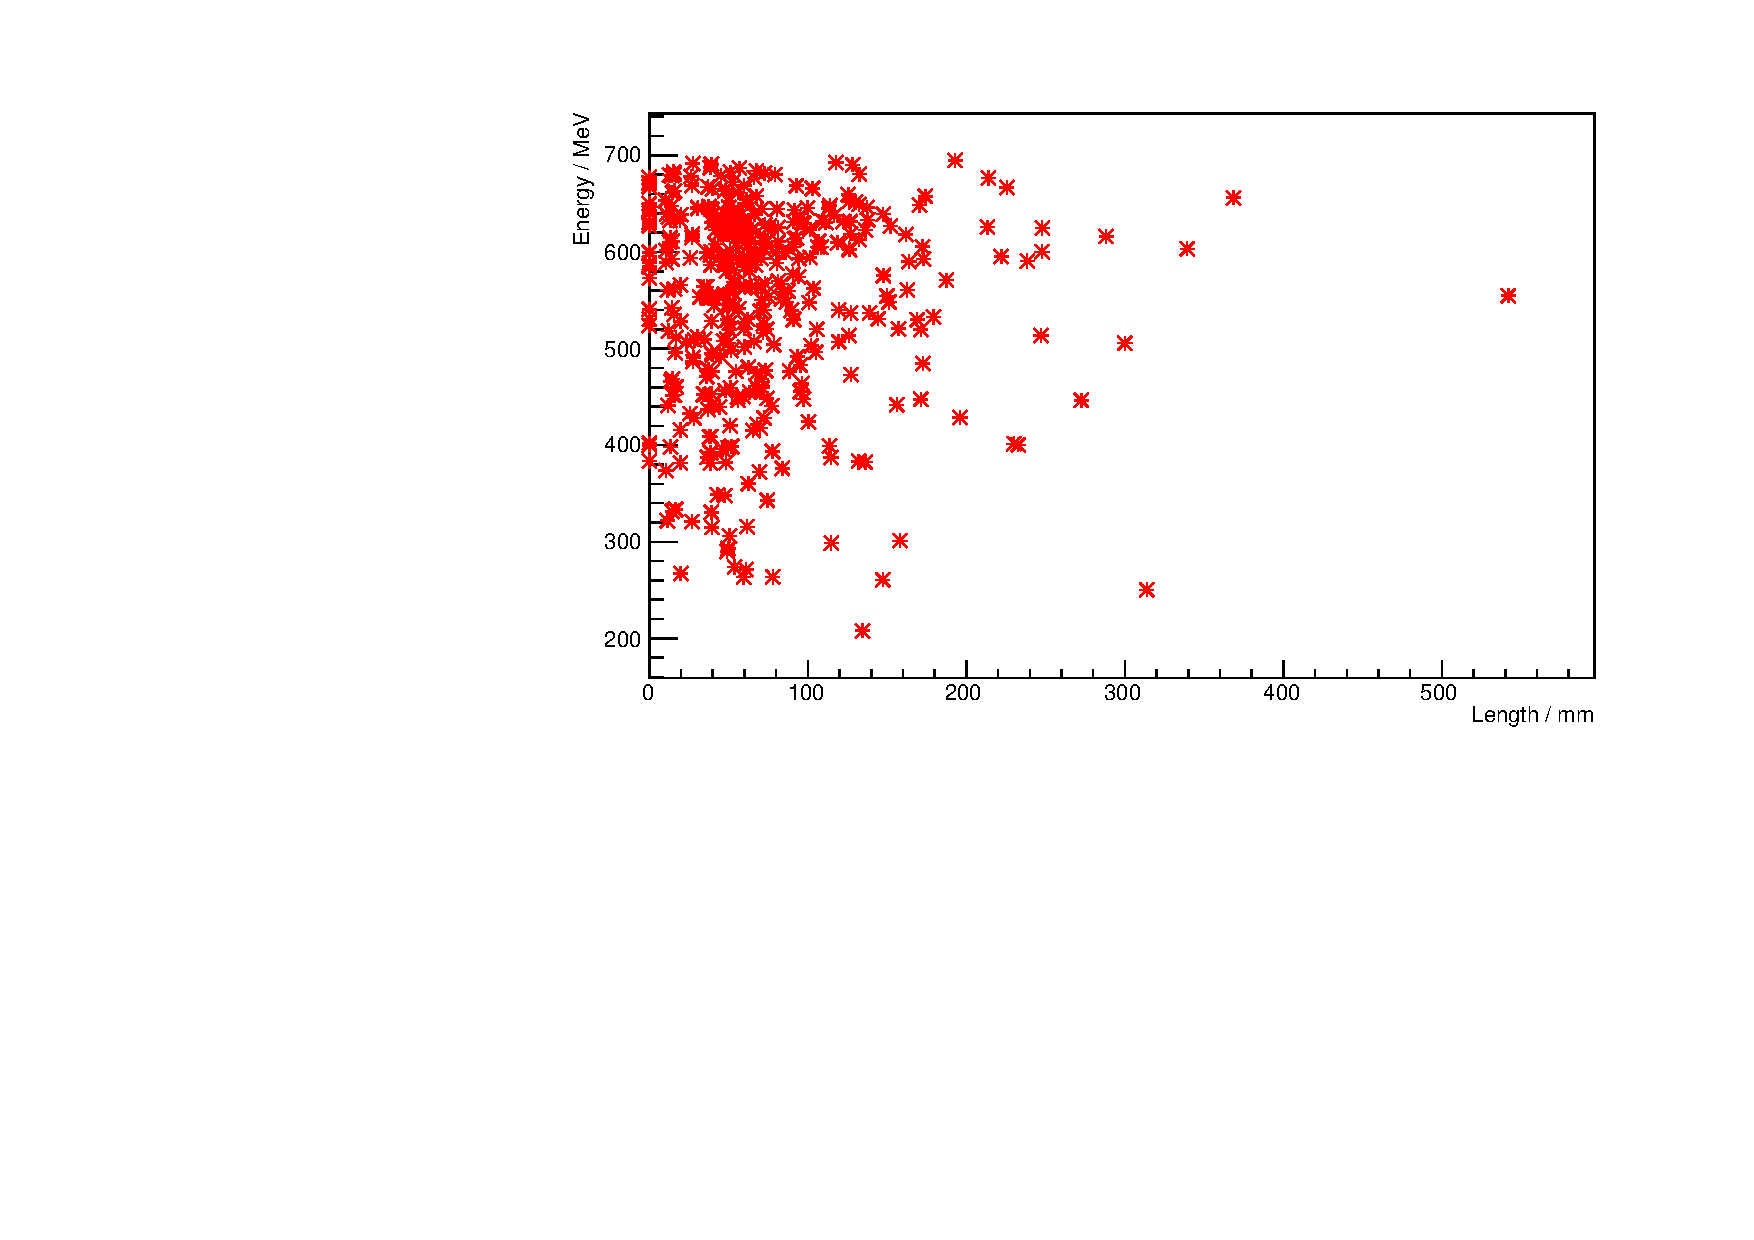
\includegraphics[angle=-90,width=0.45\textwidth]{chapters/analysis_images/seg-20}
    }
    \subfigure[$50\mm$]{
        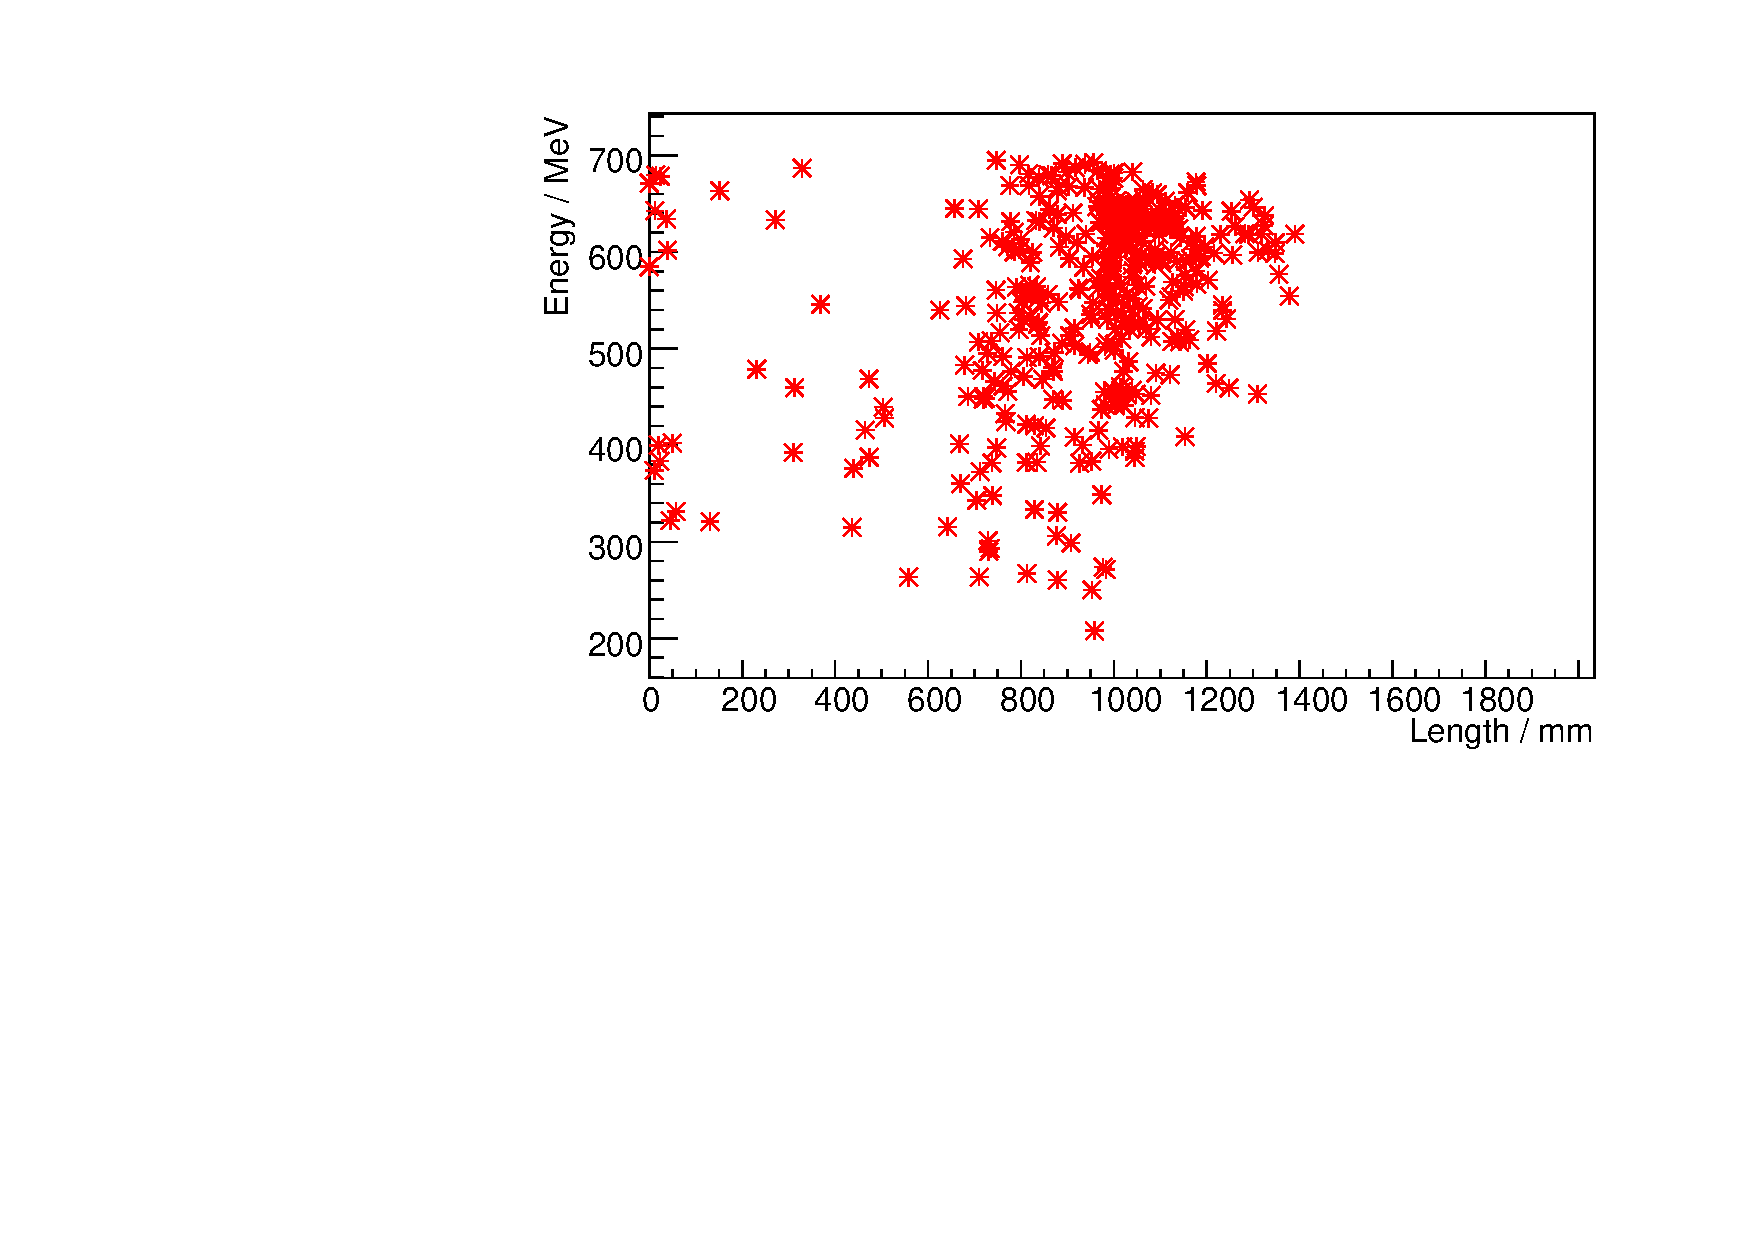
\includegraphics[angle=-90,width=0.45\textwidth]{chapters/analysis_images/seg-50}
    }
    \subfigure[$100\mm$]{
        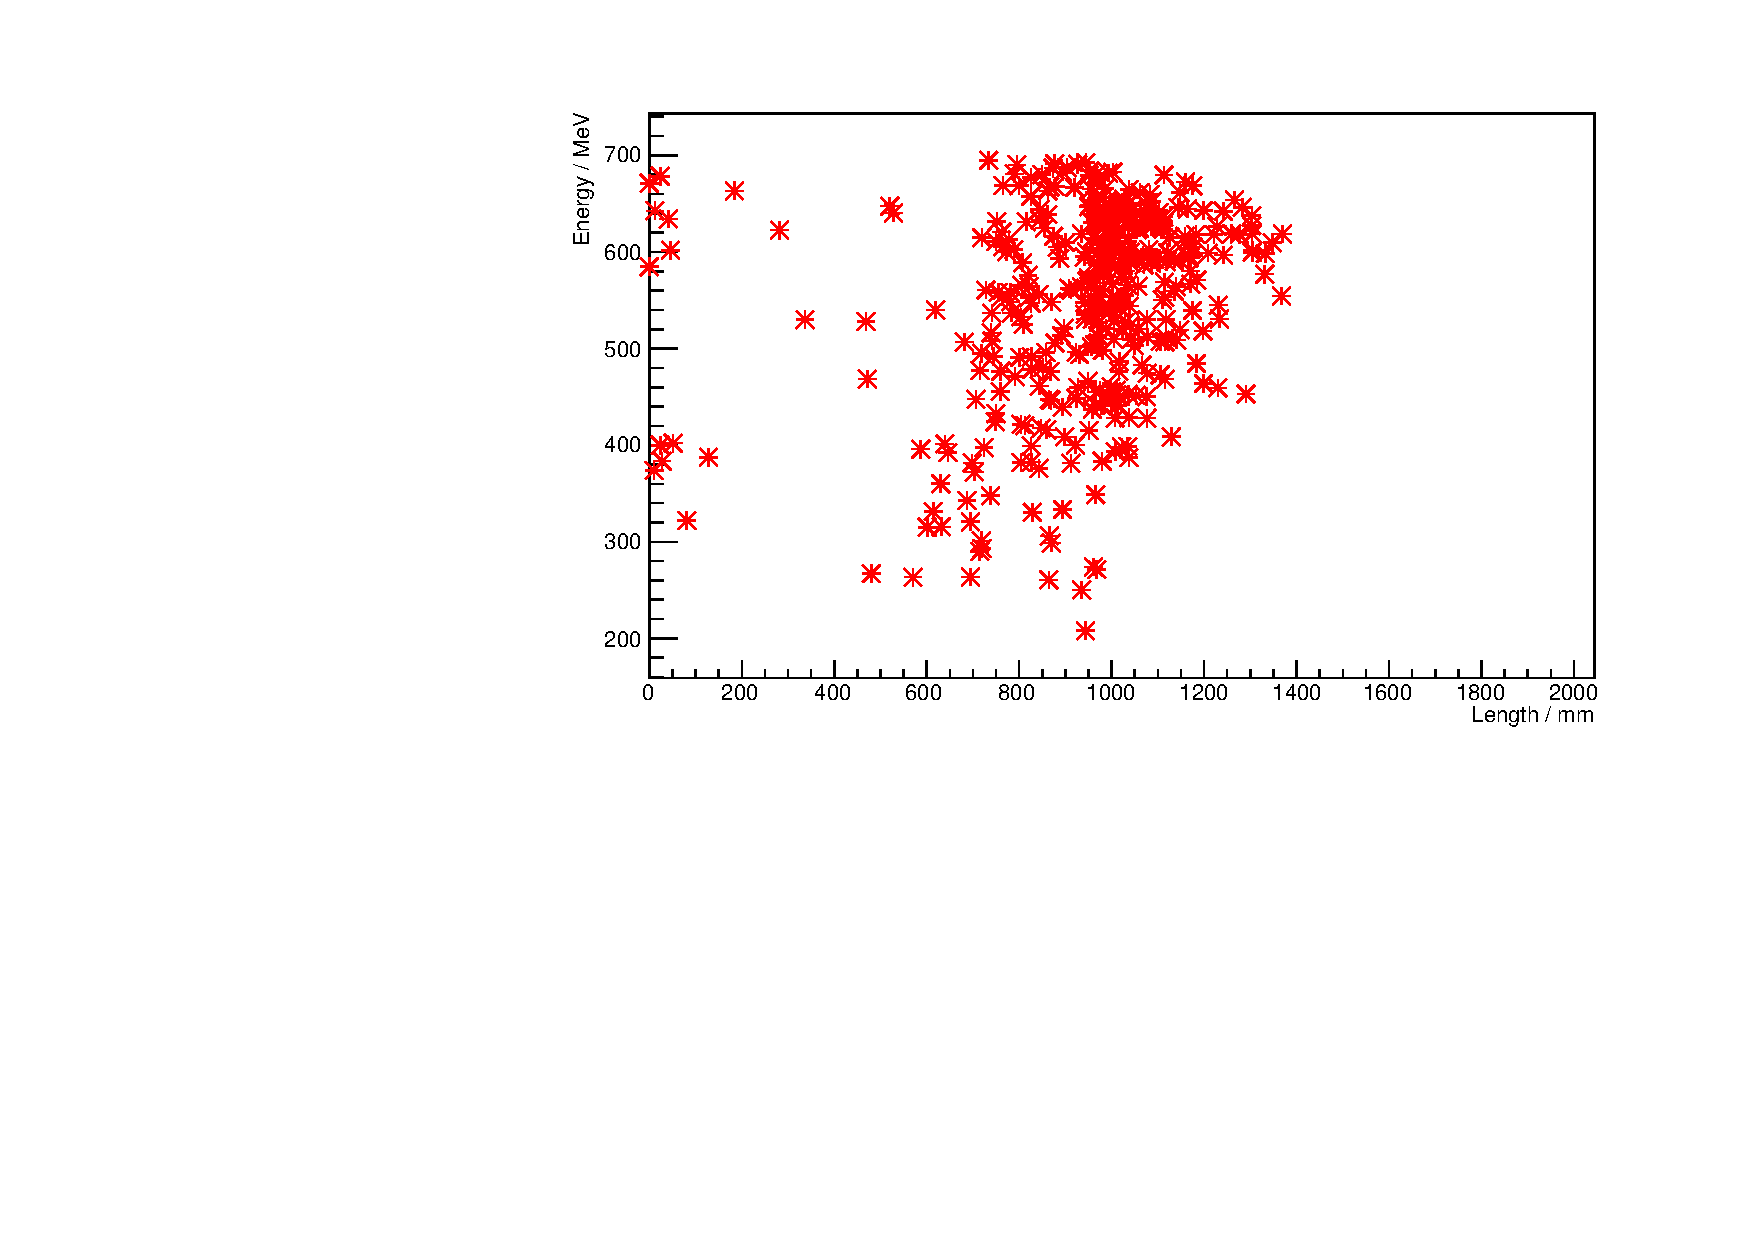
\includegraphics[angle=-90,width=0.45\textwidth]{chapters/analysis_images/seg-100}
    }
    \subfigure[$150\mm$]{
        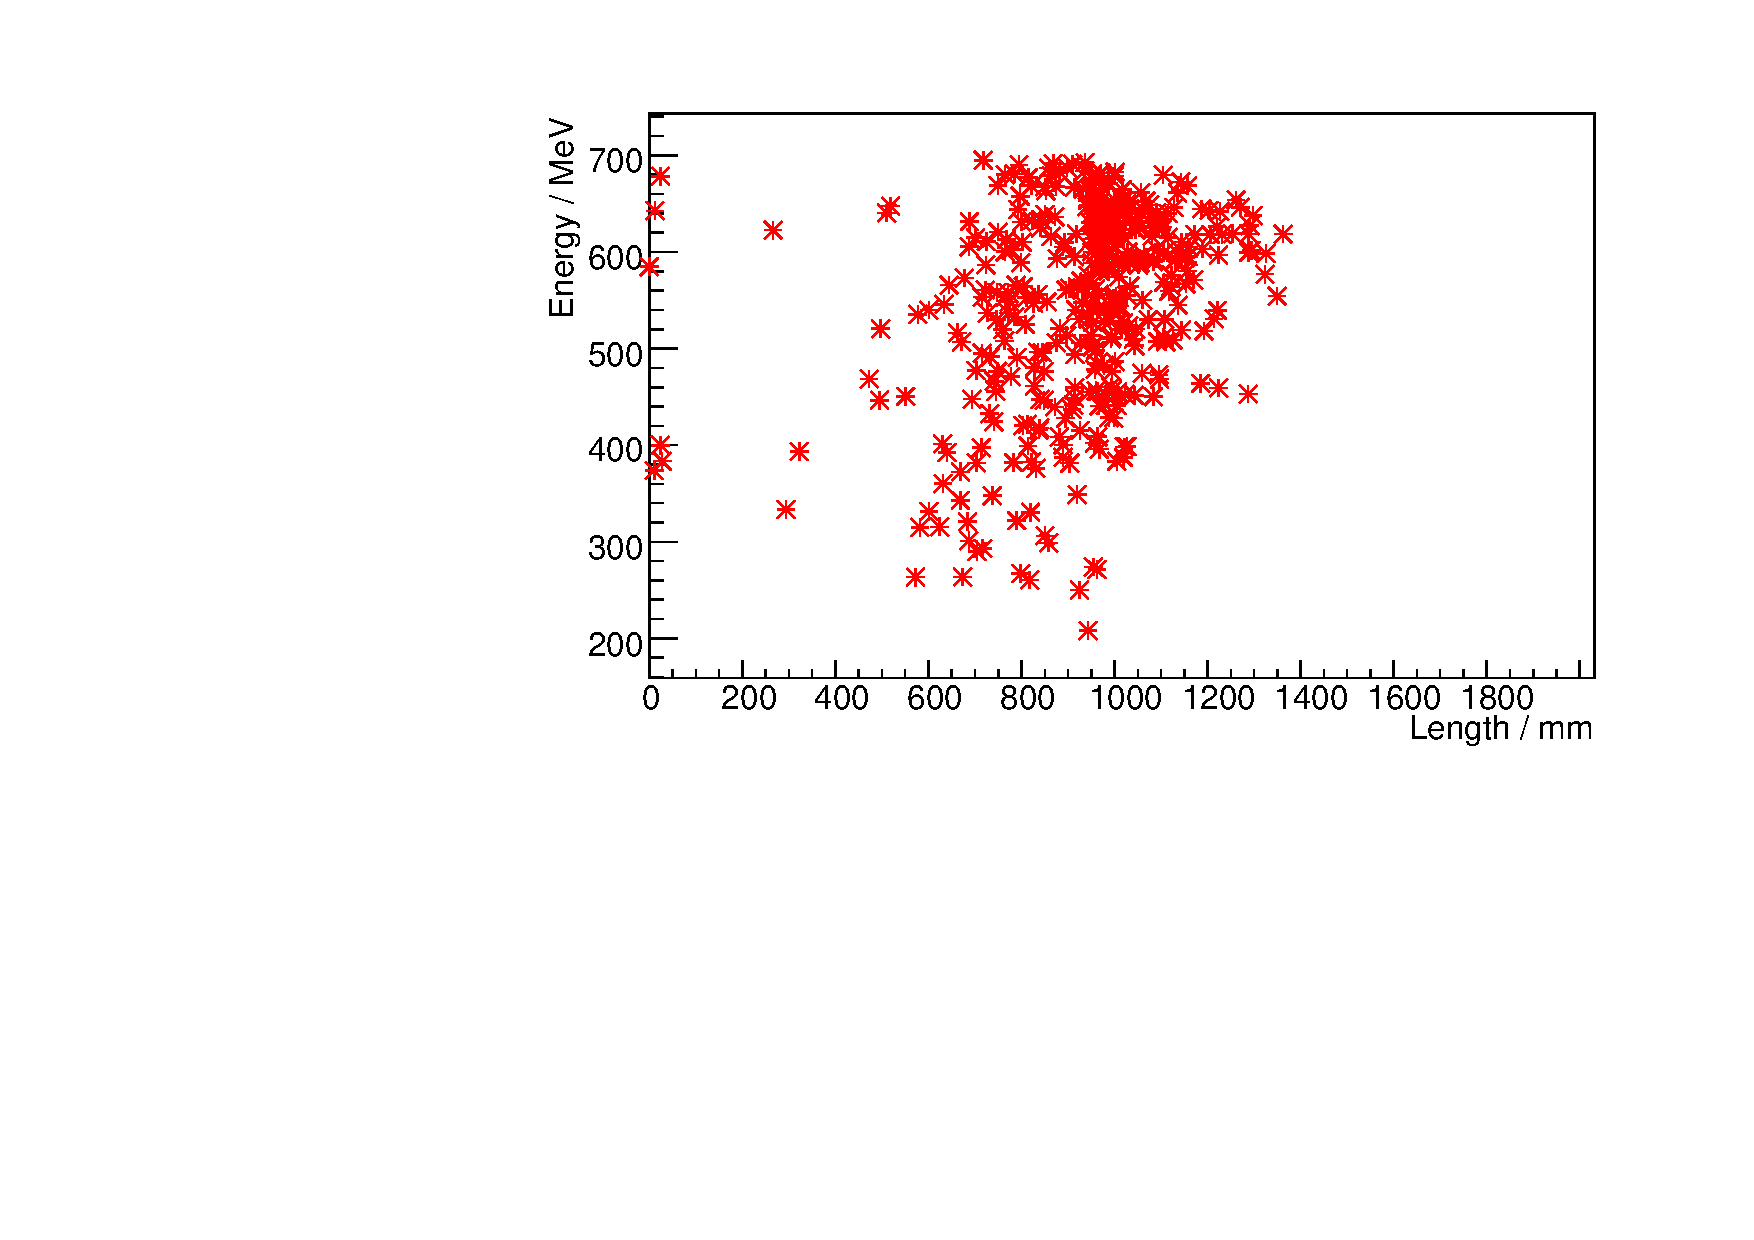
\includegraphics[angle=-90,width=0.45\textwidth]{chapters/analysis_images/seg-150}
    }
    \subfigure[$200\mm$]{
        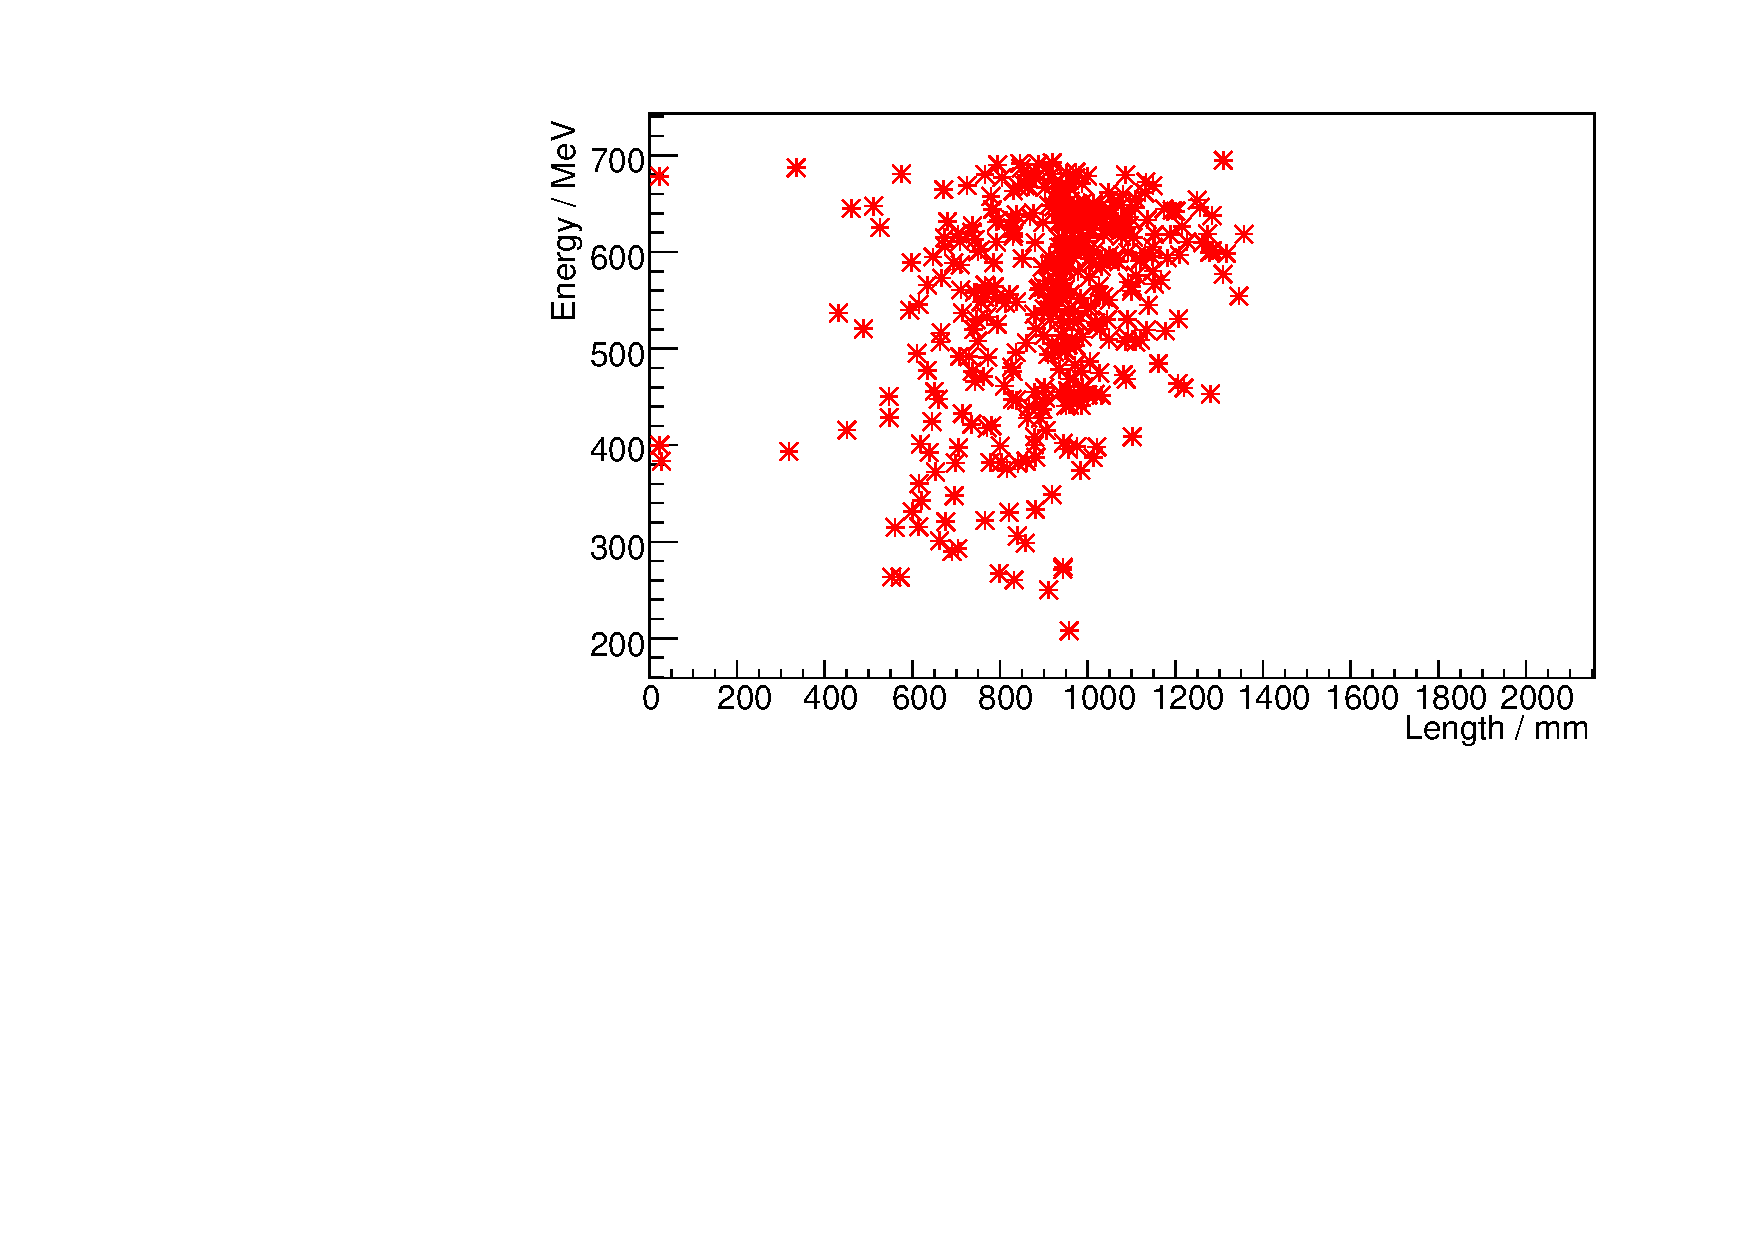
\includegraphics[angle=-90,width=0.45\textwidth]{chapters/analysis_images/seg-200}
    }
    \subfigure[$300\mm$]{
        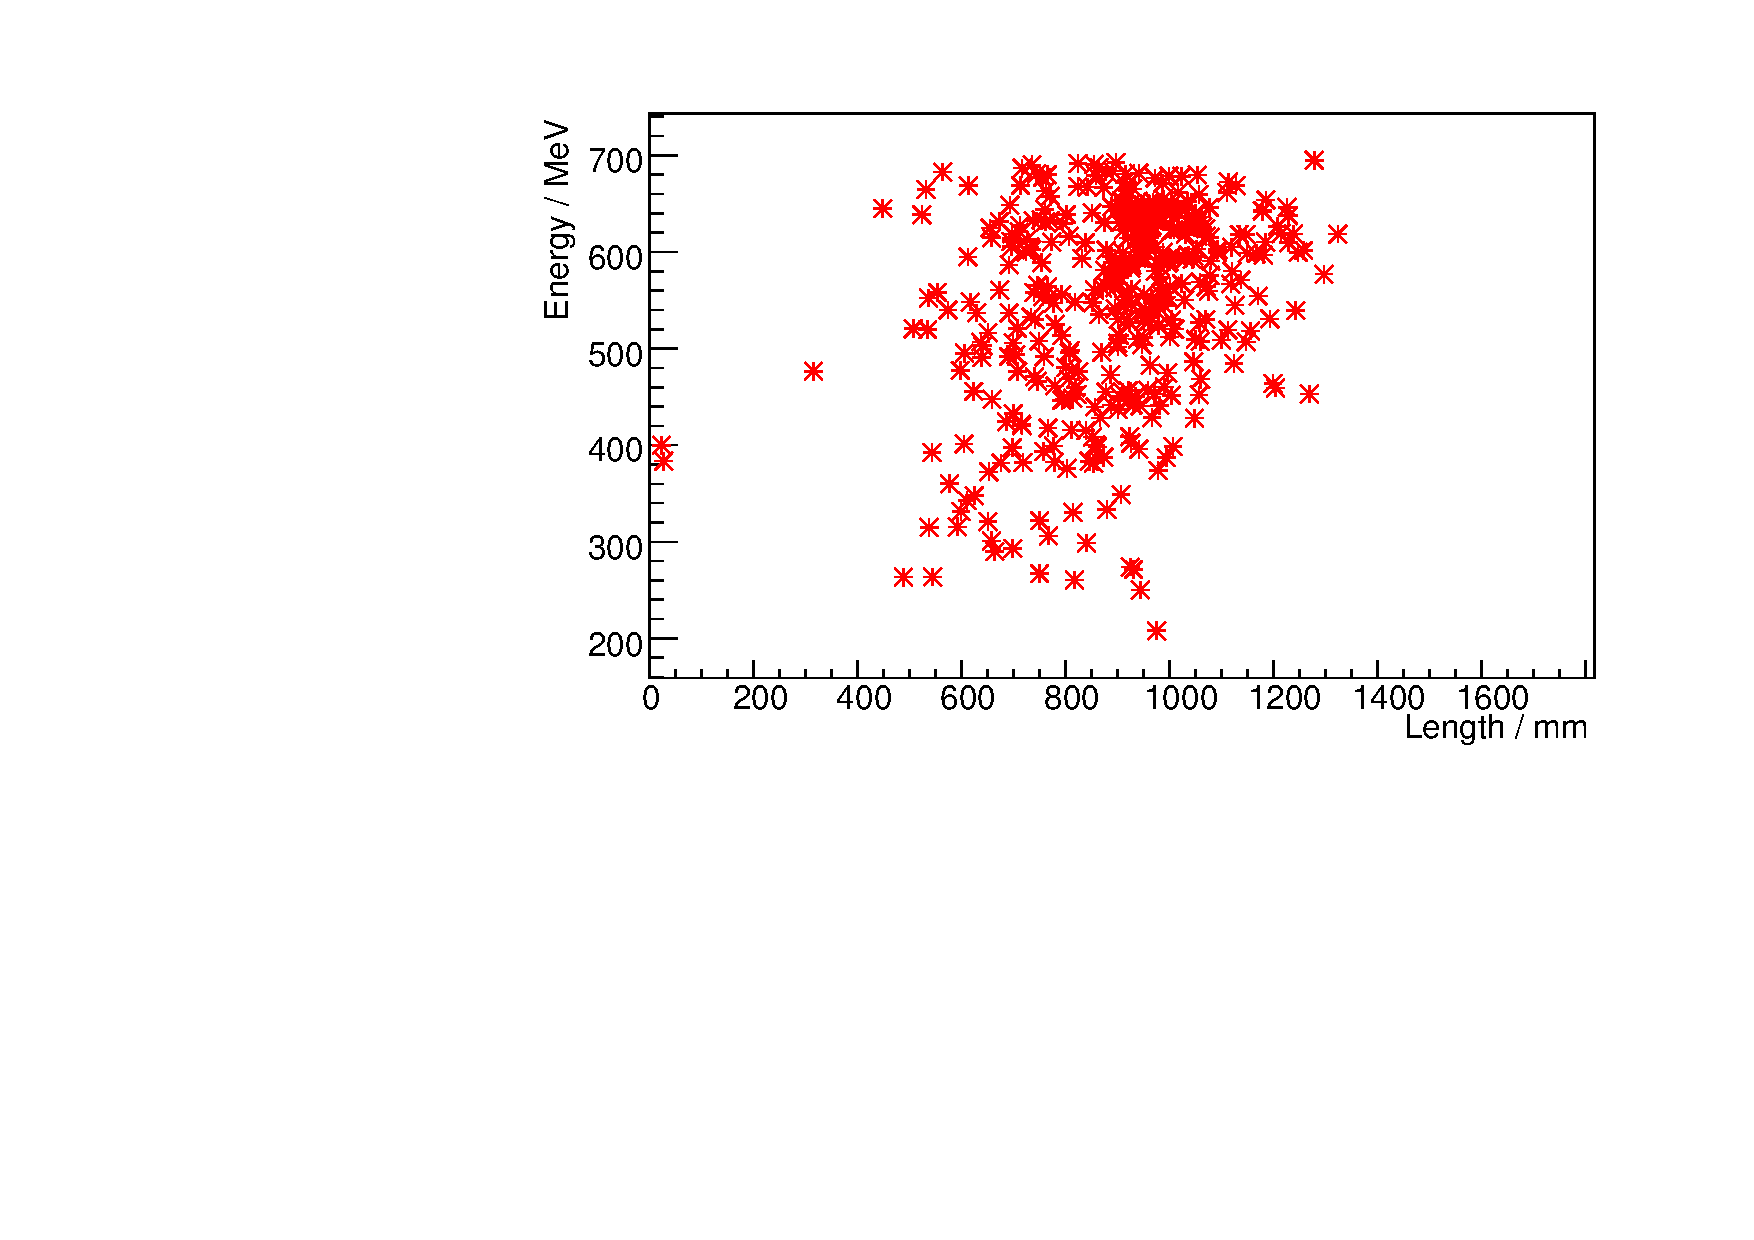
\includegraphics[angle=-90,width=0.45\textwidth]{chapters/analysis_images/seg-300}
    }
    \subfigure[$400\mm$]{
        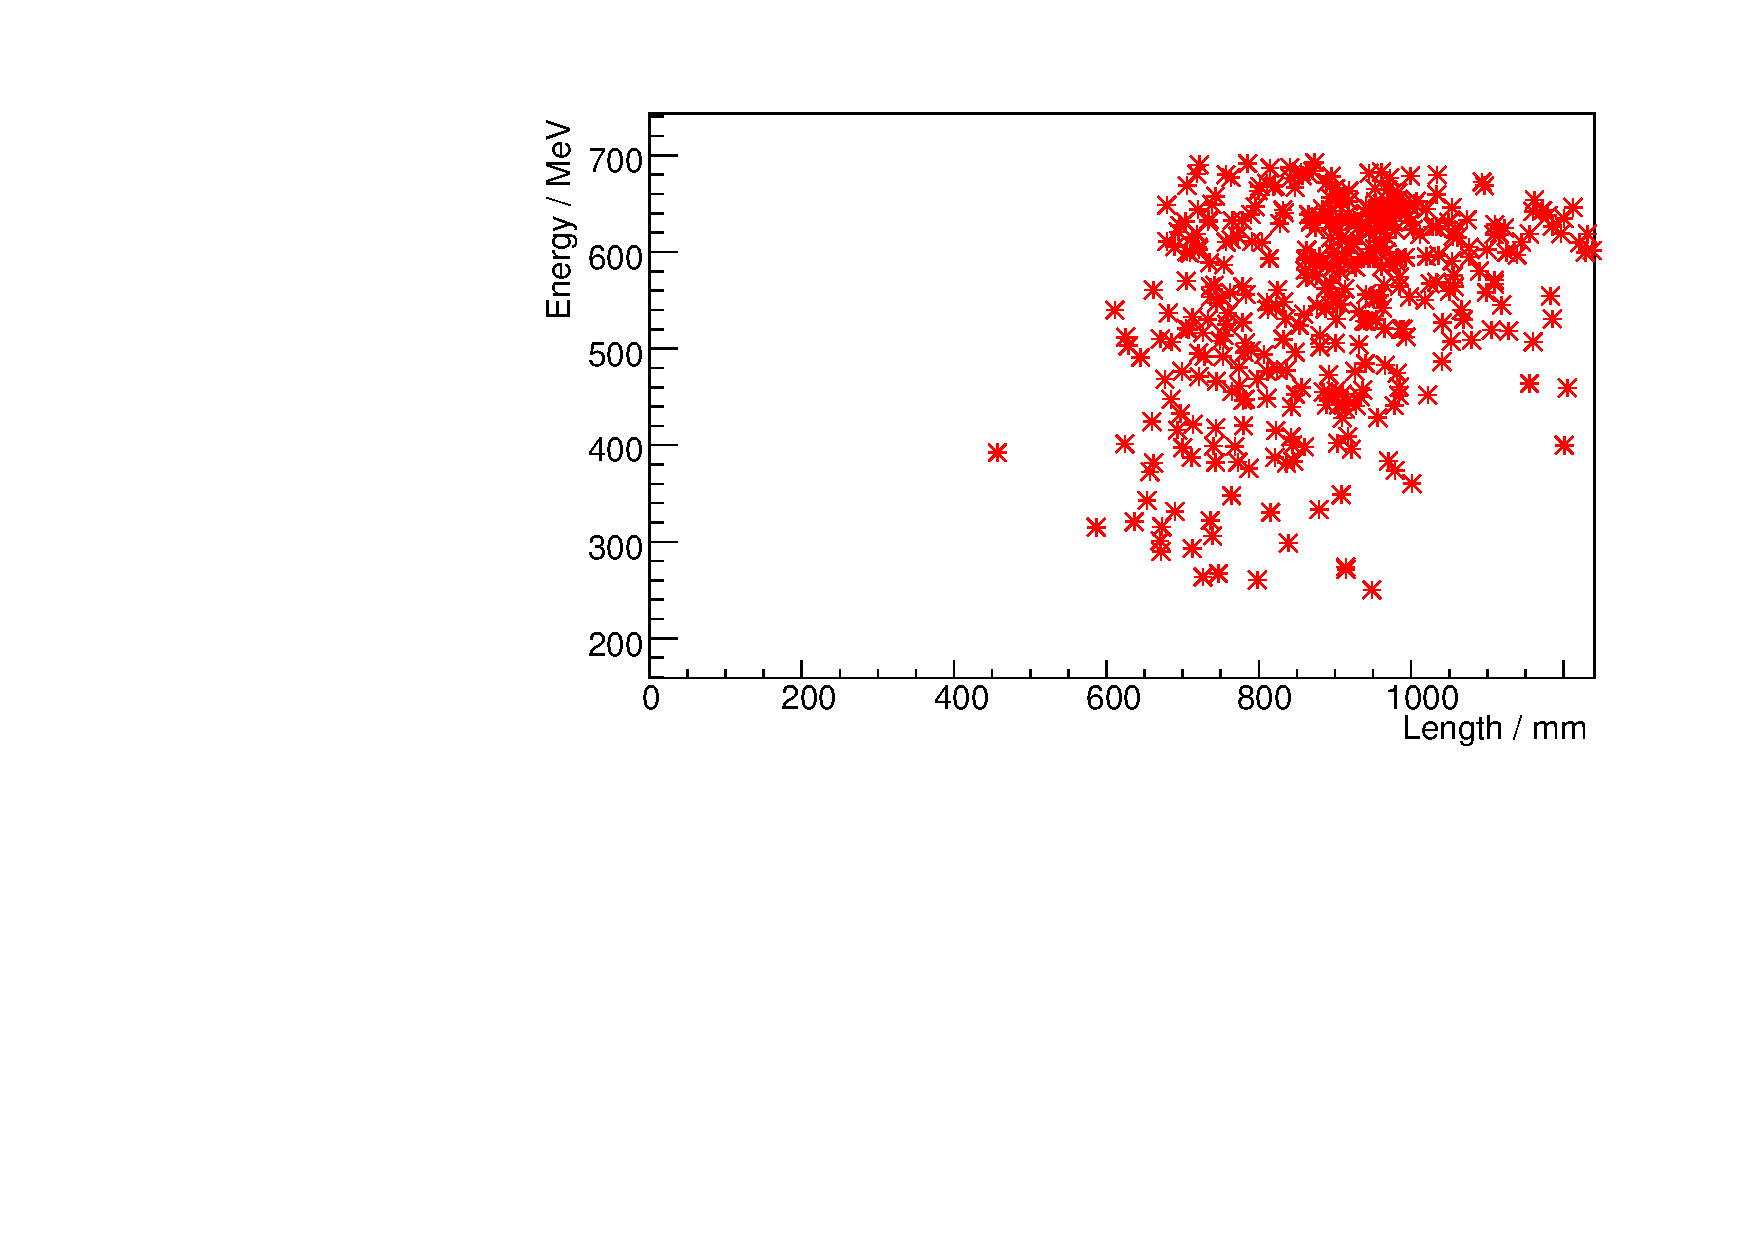
\includegraphics[angle=-90,width=0.45\textwidth]{chapters/analysis_images/seg-400}
    }
    \caption[Relationship between track length and muon energy]{\label{fig:energy-recon-track-length}Relationship between the measured length of a reconstructed track and the true energy of the corresponding muon, shown for segment lengths of $20\mm$, 50\mm$, 100\mm$, 150\mm$, 200\mm$, $300\mm$ and $400\mm$. See text for discussion.}    
\end{figure}

The track length is calculated by taking the clustered set of hits, looking for an \emph{extreme} hit, i.e. one end of the track, then searching for neighbours within some radius $R$. The furthest neighbour becomes the next seed point, and the distance between the two is added to an accumulator variable. This process is repeated, using principal components analysis to ensure that the discovered point is always moving away from the previous steps, until the other end of the track is reached. The sum of step lengths approximates the length of the entire track. The maximum segment length is determined by the value of $R$, and the results of applying this procedure to the $397$ tracks being analysed here are shown in figure \ref{fig:energy-recon-track-length} for seven different maximum segment lengths.

Smaller segment lengths allow for a more accurate estimate of the track length in the presence of curvature, but are more susceptible to gaps in the reconstructed track causing early termination of the algorithm. This can be seen in the results for a $20\mm$ segment length, where most measurements have very small lengths. Longer segment lengths are more tolerant of gaps, but provide poor estimates when traversing curved tracks, as well as reducing the sensitivity to features on a scale smaller than the segment length. This can be seen across the set of graphs, with the cluster of points shifting rightward (i.e. towards longer estimates) with increasing segment length. The results in figure \ref{fig:energy-recon-track-length} indicate that, once again, the correlation between reconstructed track length and true muon energy is poor, and cannot be used to calibrate for energy reconstruction.

\section{Conclusions}
